\documentclass{article}
\usepackage{graphicx} % new way of doing eps files
\usepackage{listings} % nice code layout
\usepackage[usenames]{color} % color
\definecolor{listinggray}{gray}{0.9}
\definecolor{graphgray}{gray}{0.7}
\definecolor{ans}{rgb}{1,0,0}
\definecolor{blue}{rgb}{0,0,1}
% \Verilog{title}{label}{file}
\graphicspath{ {H:/ELC3338/Team8/CompOrg_Spring2018_S1_Team8/images/} }
\newcommand{\Verilog}[3]{
  \lstset{language=Verilog}
  \lstset{backgroundcolor=\color{listinggray},rulecolor=\color{blue}}
  \lstset{linewidth=\textwidth}
  \lstset{commentstyle=\textit, stringstyle=\upshape,showspaces=false}
  \lstset{frame=tb}
  \lstinputlisting[caption={#1},label={#2}]{#3}
}


\author{Matthew Carrano and Breana Leal}
\title{Lab 3}

\begin{document}
\maketitle

\section{Introduction}
The goal of this lab is to create an instruction memory module, and then combine said module with previous modules to form the fetch stage module.  The instruction memory module outputs data determined by the input address. The fetch stage module uses the instruction memory module in conjunction with an adder, mux and program counter (a register module). In the fetch stage, by using the select of the mux, the program counter will either give an address to the instruction memory that is sequential or a branch value. Then the respective data will be outputted.


\section{Interface}
The inputs of the instruction memory module are clk and pc. The clk is simply a pulse with a period of 10ns. With each positive pulse edge, the pc will increment, which will affect the output. This will be explained further in implementation. 

The inputs of the iFetch are clk, reset, pc\_src, and branch\_target. The outputs of the iFetch are incremented\_pc, instruction, and cur\_pc. Its inputs and outputs serve as connecting pieces for the previously discussed modules: mux, program counter, adder, and instruction memory.

The modules in iFetch are connected as follows. incremented\_pc is the output of the adder, and thus the incremented value of the current program counter address (cur\_pc). incremented\_pc is also an input of the mux. The other input of the mux is branch\_target.  pc\_src is the select signal of the mux. The output from the mux is the input of the program counter (this is a wire called new\_pc) along with inputs clk and reset. As mentioned, the output of the program counter is cur\_pc. cur\_pc becomes an input for the adder module.The adder's other input is STEP, a parameter defined as 'WORD'd4; this equals 4 in decimal. cur\_pc and clk are inputs of the instruction memory. They lead to the output called instruction.


\section{Design}
The first module to build is the instruction memory module. The instruction memory module is designed to take one 64-bit input value and produce a 32-bit output value from a data file.

The second module to build is the iFetch module. The iFetch module needs to be the instruction memory module with the added functionality of automatically increasing the program counter value by 4, and the option to branch to a specified address. 


\section{Implementation}
The instruction memory module is implemented with a 32-bit data reg called imem. in The initial block seen in Listing 1, imem is set equal to the data in Figure 1. Creating a vector of length 18. The output, instruction, is equal to the value of imem at the index of the pc input divided by 4.  For example, if the pc input is 8, the instruction will output the binary code at line 2 from the data file.

\Verilog{Verilog code for implementing the instruction memory module.}{code:adder}{../code/1_fetch/instr_mem.v}

The iFetch module is implemented by instantiating the mux, register, adder, and instruction memory modules, and then connecting all the inputs and outputs as described in Interface. The mux is altered to have a WORD parameter and instruction memory is altered to have SIZE parameter.  cur\_pc does not have to be an output, but is set as one, so that we can see it in the timing diagram. The new\_pc wire is not set as an output because we do not need to see its value. 

\Verilog{Verilog code for implementing the iFetch module.}{code:mux}{../code/1_fetch/iFetch.v}

\section{Test Bench Design}
A test bench was made for each module. The instruction memory test bench creates a wire for the input clock (clk), and 32 bit wire for the instruction output (inst). A 64 bit reg is created for the program counter input (p\_c). An oscillator module called clock\_gen is instantiated. This generates a clock pulse on clk. An instruction memory module called UUT is then instantiated. In the initial block, the p\_c is set from 0 to 52 with increments of 4 and delays of 1 cycle (10ns) in between each increment. This simulates the incrementation of the program counter by the adder in the fetch stage. The instruction data used for testing is shown in Figure 1, with the decimal values to the right of each binary value. Only the binary values were present at testing. The results of the test are verified if the output of the module (inst) is the value at the address specified by the p\_c. For example, at p\_c equal to 0, the output should be 4165927241 because this is the data at the 0 address of the test data file. All of the code used for the instruction memory testing is in Listing~\ref{code:instrtest}.

\begin{figure}[h]
	\caption{Instruction Memory Test Data.}
	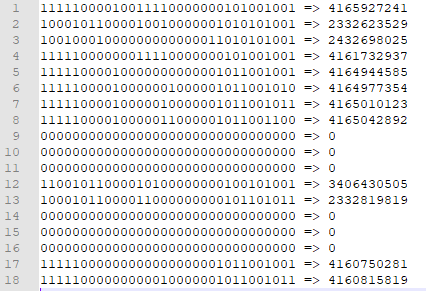
\includegraphics[scale=.85]{instr_test_data}
	\centering
\end{figure}

\Verilog{Verilog code for testing the fetch stage.}{code:instrtest}{../code/1_fetch/instr_mem_test.v} 

Next, a test bench was created for the fetch module. This required the creation of a wire called clk, a rst and pc\_s reg, a 64 bit branch reg, a 64 bit inc\_pc wire, a 32 bit instr wire, and a 64 bit c\_pc wire. Another oscillator module was instantiated, and then a iFetch module called UUT was also instantiated. To test functionality, first, the pc\_s was set with a blocking statement to 0 in order to perform sequential stepping. The reset reg is set to 0 with a non-blocking statement. This set the program counter to an initial value of 0. Then a delay of 4 cycles occurs. With these three lines of code we can verify that the sequential fetching works correctly. In the simulation we should see the program counter start at 0 and increment by 4. As this is happening the respective instructions should be outputted (the same instruction data was used). After the 4 cycles are finished the pc\_s is set to 1 and the branch is set to 4. A delay of 2 cycles is added. This is used to verify that the branching functionality works. We should see the program counter change to 4 at a positive clock edge, and then stay at 4 until the pc\_s is set back to 0. When p\_c is set back to 0, the program counter will resume stepping by 4 starting with the branch value. All of the code used for the iFetch testing is in Listing~\ref{code:fetchtest}.

\Verilog{Verilog code for testing the fetch stage.}{code:fetchtest}{../code/1_fetch/iFetch_test.v}

\section{Simulation}
The timing diagrams in Figure 2 and 3 verify that both modules work as detailed in the above section. One way to easily verify functionality is to compare the outputs to the data of Figure 1.

\begin{figure}[h]	
	\caption{Timing diagram for instruction module test.}
	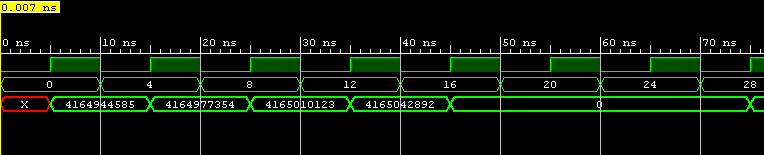
\includegraphics[width=\textwidth]{instr_memSim1}
	\label{fig:instrmemtest}
\end{figure}

\begin{figure}[h]	
	\caption{Timing diagram for fetch module test.}
	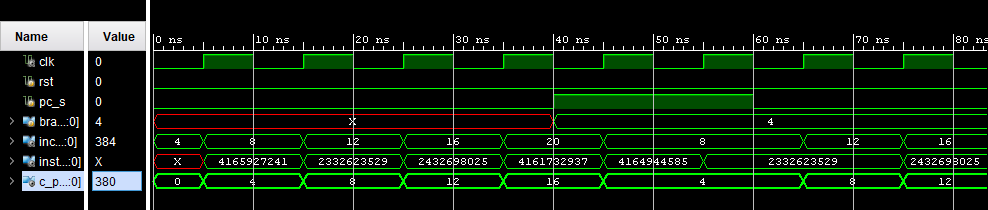
\includegraphics[width=\textwidth]{fetch_sim}
	\label{fig:fetchtest}
\end{figure}


\section{Conclusions}
The instruction module and fetch module were successfully established.  The instruction memory module is used in conjunction with the mux, register, and adder modules to create the fetch. With the fetch module, we can read and output data sequentially or through a branch. 

\end{document} 